\chapter{Arhitektura i dizajn sustava}


Sve web aplikacije sastavljene su od klijentske strane(eng.frontend) i od serverske strane(eng.backend). Kod u klijentskoj strani je pisan u HTML, CSS i JS i on se izvodi u web pregledniku. Dok serverska strana se sastoji od poslovne logike i koda koji odgovara na HTTP zahtjeve. Kod na serverskoj strani može biti pisan u Javi, PHP, Python, itd.



\begin{figure}[H]
	
	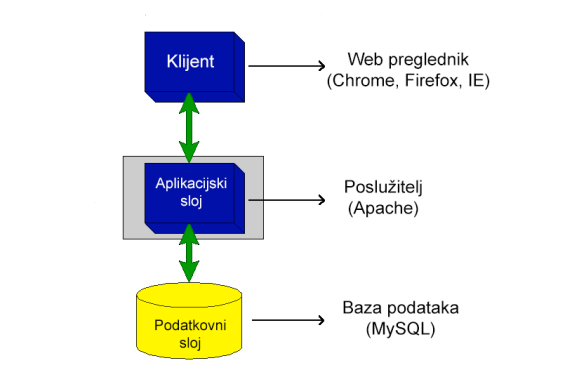
\includegraphics[width=\textwidth]{slike/webAplikacija.png} %veličina slike u odnosu na originalnu datoteku i pozicija slike
	\centering
	\caption{Arhitektura web aplikacije}
	\label{fig:arhitekturaWebApp}
\end{figure}
Web aplikacije podijeljene su na tri glavna sloja:

\begin{itemize}
	\item \textbf{Prvi sloj predstavlja prezentacijski sloj}, to je korisničko sučelje i komunikacijski sloj aplikacije gdje korisnik stupa u interakciju s aplikacijom. Glavna svrha prezentacijskog sloja je prikazivanje i prikupljanje informacija od korisnika.
	\item\textbf{Drugi sloj predstavlja aplikacijski sloj}, je glavni sloj web aplikacije. U ovom sloju se informacije prikupljene u prezentacijskom sloju obrađuju korištenjem poslovne logike. Te se također u ovom sloju dohvaćaju unose i izmjenjuju podatci koji se nalaze u podatkovnom sloju
	\item\textbf{Treći sloj je podatkovni sloj}, ili baza podataka je sloj u kojem se pohranjuju podatci koje koristi o obrađuje web aplikacija i u kojem se pristupa istim.
\end{itemize} 

Svi slojevi međusobno komuniciraju preko standardiziranih Internetskih protokola, kojih se prilikom razvoja 
aplikacija treba pridržavati.Glavne prednosti razvijanja aplikacija u tri sloja su:
\begin{itemize}
	\item Svaki sloj može biti napravljen u različitom programskom jeziku i okruženju.
	\item Svaki sloj može biti pokrenut na vlastitom serveru sto znači da slojevi ne ovise jedan o drugom.
	\item Brži razvoj aplikacije zato sto se svaki sloj može razvijati istovremeno.
	\item Poboljšana sigurnost zato sto možemo vršiti provjeru nad upitima i podatcima na tri razine i zbog toga što korisnik ne radi direktno sa SQL serverom.
\end{itemize}
Programski jezik kojeg smo odabrali za izradu naše web aplikacije je Java zajedno s Spring Boot-om i Thymeleaf-om. 
Odabrano razvojno okruženje je IntelliJ IDEA. Arhitektura sustava temeljiti  će se na MVC 
(Model-View-Controller) konceptu. MVC koncept podržan je od strane Spring Boot radnog okvira i kao takav ima gotove predloške koji nam olakšavaju razvoj web aplikacije.
MVC koncept sastoji se od:
\begin{itemize}
	\item \textbf{Model} - Komponenta Model sadrzi cijelu logiku vezanu za podatke s kojom korisnik radi. To mogu biti podatci koji se prenose između komponenti View i Controler ili bilo koje druge podatke vezane za poslovnu logiku.
	\item \textbf{View} - Komponenta View koristi se za svu logiku korisničkog sučelja aplikacije.  Na primjer, korisnički prikaz uključivat će sve komponente korisničkog sučelja kao što su tekstualni okviri, padajući izbornik itd. s kojima je u interakciji krajnji korisnik.
	\item \textbf{Controller} - Kontroleri djeluju kao sučelje između komponenti Modela i Viewa za obradu sve poslovne logike i dolaznih zahtjeva, manipuliranje podacima pomoću komponente Model i interakciju s Viewsima kako bi prikazali konačni izlaz.
\end{itemize} 
\eject


\section{Baza podataka}


Za našu web aplikaciju koristit ćemo relacijsku bazu podataka. Relacijska model baze podataka se sastoji od više tablica podataka takozvanih relacija. Svaka relacija ima svoje ime koje je jedinstveno u toj bazi podataka i koristimo ga za razlikovanje relacija u jednoj bazi podataka. Svaka relacija ima stupce koji sadrže vrijednost nekog atributa. Atribut ima svoje ime po kojem ga razlikujemo od drugih atributa u toj relaciji. Svaka tablica ima jedan ili više jednistvenih atributa ili skup atributa koji je jedinstven koji se koristi kao primarni ključ tablice. Entiteti u našoj bazi podataka su:

\begin{itemize}
	\item \textbf{Korisnik}(usertable)
	\item \textbf{Voditelj parkinga}(parkingowner)
	\item \textbf{Klijent}(client)
	\item \textbf{Rezervacija}(clientreservation)
	\item \textbf{Parkiralište}(parking)
	\item \textbf{Parkirališno mjesto}(parkingspot)
	\item \textbf{Zauzetost parkirnog mjesta}(parkingspotoccupancy)
\end{itemize}



\subsection{Opis tablica}


\textbf{Korisnik}  Ovaj entitet sadrži sve važne informacije o korisniku aplikacije. Sadrži atribute: identifikator korisnika, korisničko ime, ime, prezime, email korisnika, lozinku, tip korisnika aplikacije i oznaku je li administrator potvrdio taj korisnički račun. Ovaj entitet ima dvije specijalizacije na klijenta i voditelja parkinga.
\begin{longtblr}[
	label=none,
	entry=none
	]{
		width = \textwidth,
		colspec={|X[6,l]|X[6, l]|X[20, l]|}, 
		rowhead = 1,
	} %definicija širine tablice, širine stupaca, poravnanje i broja redaka naslova tablice
	\hline \multicolumn{3}{|c|}{\textbf{Korisnik(usertable)}}	 \\ \hline[3pt]
	\SetCell{LightGreen}userid & INT	&  	Jedinstveni identifikator korisnika  	\\ \hline
	username	& VARCHAR &   Korisničko ime	\\ \hline 
	userfirstname & VARCHAR & Ime korisnika  \\ \hline 
	usersurename & VARCHAR	&  Prezime korisnika		\\ \hline 
	useremail & VARCHAR & Email korinika \\ \hline
	temppassword & VARCHAR & Privremena lozinka \\ \hline
	usertype & VARCHAR & Tip korisnika aplikacije (voditelj ili klijent)\\\hline
	confirmed & BOOLEAN & Varijabla koja pokazuje je li korisnik potvrđen od strane administratora \\\hline
\end{longtblr}

\textbf{Voditelj parkirališta}  Ovaj entitet je specijalizacija entiteta korisnik on sadrži dodatne atribute: iban i poveznicu na sliku osobne iskaznice. Povezan je sa parkiralištem vezom n naprema n.
\begin{longtblr}[
	label=none,
	entry=none
	]{
		width = \textwidth,
		colspec={|X[6,l]|X[6, l]|X[20, l]|}, 
		rowhead = 1,
	} %definicija širine tablice, širine stupaca, poravnanje i broja redaka naslova tablice
	\hline \multicolumn{3}{|c|}{\textbf{Voditelj parkirališta(parkingowner)}}\\ \hline[3pt]
	\SetCell{LightGreen}userid & INT	&  	Jedinstveni identifikator korisnika  	\\ \hline
	iban	& CHARACTER &   IBAN vlasnika parkinga	\\ \hline 
	idpicture & VARCHAR &  Poveznica na sliku osobne iskaznice \\ \hline 
\end{longtblr}

\textbf{Klijent}  Ovaj entitet je specijalizacija entiteta korisnik on sadrži dodatni atribut stanje računa klijenta. Povezan je sa entitetom rezervacija vezom n naprema n.
\begin{longtblr}[
	label=none,
	entry=none
	]{
		width = \textwidth,
		colspec={|X[6,l]|X[6, l]|X[20, l]|}, 
		rowhead = 1,
	} %definicija širine tablice, širine stupaca, poravnanje i broja redaka naslova tablice
	\hline \multicolumn{3}{|c|}{\textbf{Klijent(client)}}\\ \hline[3pt]
	\SetCell{LightGreen}userid & INT	&  	Jedinstveni identifikator korisnika  	\\ \hline
	walletbalance	& NUMERIC &   Stanje računa klijenta	\\ \hline 
\end{longtblr}

\textbf{Parkiralište}  Ovaj entitet sadrži sve bitne informacije o parkiralištu. Atributi su mu: korisnički id voditelja parkirališta, ime parkinga, poveznica na sliku parkinga, cijena parkinga po satu i opis parkirališta. Povezan je sa voditeljem parkiralista vezom n naprema n i sa parkirališnim mjestom vezom n naprema n. 
\begin{longtblr}[
	label=none,
	entry=none
	]{
		width = \textwidth,
		colspec={|X[6,l]|X[6, l]|X[20, l]|}, 
		rowhead = 1,
	} %definicija širine tablice, širine stupaca, poravnanje i broja redaka naslova tablice
	\hline \multicolumn{3}{|c|}{\textbf{Parkiralište(parking)}}	 \\ \hline[3pt]
	\SetCell{LightGreen}userid & INT	&  	Jedinstveni identifikator voditelja parkinga  	\\ \hline
	parkingname	& VARCHAR &   Ime parkirališta	\\ \hline 
	parkingphoto & VARCHAR &  Poveznica na sliku parkirališta \\ \hline 
	hourlyprice & VARCHAR	&  Cijena parkiranja po satu		\\ \hline 
	description & VARCHAR &   Opis parkirališta	\\ \hline 
\end{longtblr}

\textbf{Parkirališno mjesto}  Ovaj entitet sadrži sve bitne informacije o parkirališnom mjestu. Atributi su mu: korisnički id voditelja parkirališta, broj parkirališnog mjesta na parkiralištu, tip parkirališnog mjesta, mogućnost rezervacije te x i y koordinate za 4 točke koje označavaju granice parkirališnog mjesta. Povezan je vezon n naprema n sa parkiralištem i rezervacijom a vezom 1 naprema n sa zauzetosti parkirališnog mjesta.
\begin{longtblr}[
	label=none,
	entry=none
	]{
		width = \textwidth,
		colspec={|X[10,l]|X[6, l]|X[20, l]|}, 
		rowhead = 1,
	} %definicija širine tablice, širine stupaca, poravnanje i broja redaka naslova tablice
	\hline \multicolumn{3}{|c|}{\textbf{Parkirališno mjesto(parkingspot)}}	 \\ \hline[3pt]
	\SetCell{LightGreen}userid & INT	&  	Jedinstveni identifikator voditelja parkinga  	\\ \hline
	\SetCell{LightGreen}parkingspotnumber & INT	&  	Broj parkirališnog mjesta na parkiralištu  	\\ \hline
	parkingspottype	& VARCHAR &   Vrsta parkirališnog mjesta(Za automobile ili za bicikle)	\\ \hline 
	canbereserved & BOOLEAN & Mogućnost rezerviranja parkirališnog mjesta  \\ \hline 
	pointx1 & NUMERIC & Koordinata x prve točke parkirnog mjesta\\\hline
	pointy1 & NUMERIC & Koordinata y prve točke parkirnog mjesta\\\hline
	pointx2 & NUMERIC & Koordinata x druge točke parkirnog mjesta\\\hline
	pointy2 & NUMERIC & Koordinata y druge točke parkirnog mjesta\\\hline
	pointx3 & NUMERIC & Koordinata x treće točke parkirnog mjesta\\\hline
	pointy3 & NUMERIC & Koordinata y treće točke parkirnog mjesta\\\hline
	pointx4 & NUMERIC & Koordinata x četvrte točke parkirnog mjesta\\\hline
	pointy4 & NUMERIC & Koordinata y četvrte točke parkirnog mjesta\\\hline
\end{longtblr}

\textbf{Zauzetost parkirališnog mjesta}  Ovaj entitet sadrži informacije koje se koriste za statističku analizu zauzetosti parkirališnog mjesta. Atributi su mu: korisnički id voditelja parkirališta, broj parkirališnog mjesta na parkiralištu, vrijeme od, vrijeme do i zauzetost u tom razdoblju. Povezan je vezom n naprema 1 sa parkirališnim mjestom.
\begin{longtblr}[
	label=none,
	entry=none
	]{
		width = \textwidth,
		colspec={|X[10,l]|X[6, l]|X[20, l]|}, 
		rowhead = 1,
	} %definicija širine tablice, širine stupaca, poravnanje i broja redaka naslova tablice
	\hline \multicolumn{3}{|c|}{\textbf{Zauzetost parkirnog mjesta(parkingspotoccupancy)}}	 \\ \hline[3pt]
	\SetCell{LightGreen}userid & INT	&  	Jedinstveni identifikator voditelja parkinga  	\\ \hline
	\SetCell{LightGreen}parkingspotnumber & INT	&  	Broj parkirnog mjesta na parkiralištu  	\\ \hline
	\SetCell{LightGreen}datefrom & TIMESTAMP	&  	Početak zauzetosti parkirališnog mjesta	\\ \hline
	dateto	& TIMESTAMP &  	Kraj zauzetosti parkirališnog mjesta	 	\\ \hline 
	occupancy & BOOLEAN  &  Varijabla koja nam govori da li je parkirališno mjesto bilo zauzeto \\ \hline 
\end{longtblr}
\eject
\textbf{Rezervacija}  Ovaj entitet sadrži informacije o rezervacijama parkirališnih mjesta. Sadrži atribute: jedinstveni identifikator klijenta, vrijeme početka rezervacije, jedinstveni identifikator voditelja parkinga, broj parkirnog mjesta na parkiralištu, duljina rezervacije i varijablu koja nam govori je li rezervacija ponavljajuća. Povezan je vezon n naprema n sa klijentom i sa parkirališnim mjestom.
\begin{longtblr}[
	label=none,
	entry=none
	]{
		width = \textwidth,
		colspec={|X[10,l]|X[6, l]|X[20, l]|}, 
		rowhead = 1,
	} %definicija širine tablice, širine stupaca, poravnanje i broja redaka naslova tablice
	\hline \multicolumn{3}{|c|}{\textbf{Rezervacija(clientreservation)}	 }\\ \hline[3pt]
	\SetCell{LightGreen}userid & INT	&  	Jedinstveni identifikator klijenta 	\\ \hline
	\SetCell{LightGreen}timeofstart & TIMESTAMP	&  	Vrijeme početka rezervacije  	\\ \hline
	\SetCell{LightBlue}userid & INT	&  	Jedinstveni identifikator voditelja parkinga  	\\ \hline
	\SetCell{LightBlue}parkingspotnumber & INT	&  	Broj parkirnog mjesta na parkiralištu  	\\ \hline
	duration & INT & Duljina rezervacije\\ \hline 
	reccuring & BOOLEAN & Varijabla koja definira je li rezervacija ponavljajuća \\\hline
\end{longtblr}

\subsection{Dijagram baze podataka}


\begin{figure}[H]
	
	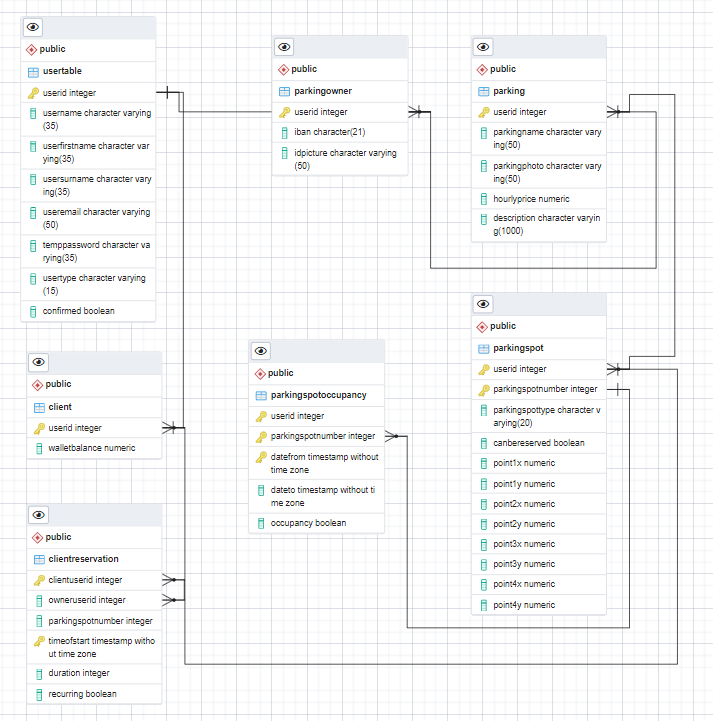
\includegraphics[width=\textwidth]{slike/db.png} %veličina slike u odnosu na originalnu datoteku i pozicija slike
	\centering
	\caption{E-R dijagram baze podataka}
	\label{fig:dijagramBP}
\end{figure}

\eject



\section{Dijagram razreda}

\textit{Potrebno je priložiti dijagram razreda s pripadajućim opisom. Zbog preglednosti je moguće dijagram razlomiti na više njih, ali moraju biti grupirani prema sličnim razinama apstrakcije i srodnim funkcionalnostima.}\\

\textbf{\textit{dio 1. revizije}}\\

\textit{Prilikom prve predaje projekta, potrebno je priložiti potpuno razrađen dijagram razreda vezan uz \textbf{generičku funkcionalnost} sustava. Ostale funkcionalnosti trebaju biti idejno razrađene u dijagramu sa sljedećim komponentama: nazivi razreda, nazivi metoda i vrste pristupa metodama (npr. javni, zaštićeni), nazivi atributa razreda, veze i odnosi između razreda.}\\

\textbf{\textit{dio 2. revizije}}\\			

\textit{Prilikom druge predaje projekta dijagram razreda i opisi moraju odgovarati stvarnom stanju implementacije}



\eject

\section{Dijagram stanja}


\textbf{\textit{dio 2. revizije}}\\

\textit{Potrebno je priložiti dijagram stanja i opisati ga. Dovoljan je jedan dijagram stanja koji prikazuje \textbf{značajan dio funkcionalnosti} sustava. Na primjer, stanja korisničkog sučelja i tijek korištenja neke ključne funkcionalnosti jesu značajan dio sustava, a registracija i prijava nisu. }


\eject 

\section{Dijagram aktivnosti}

\textbf{\textit{dio 2. revizije}}\\

\textit{Potrebno je priložiti dijagram aktivnosti s pripadajućim opisom. Dijagram aktivnosti treba prikazivati značajan dio sustava.}

\eject
\section{Dijagram komponenti}

\textbf{\textit{dio 2. revizije}}\\

\textit{Potrebno je priložiti dijagram komponenti s pripadajućim opisom. Dijagram komponenti treba prikazivati strukturu cijele aplikacije.}